\section{Evaluation}
\label{sec:egolog_evaluation}
\subsection{Experiment Setup}

\subsubsection{Implementation}
We implemented our system on a Raspberry Pi 4, which was connected to multiple devices: binaural earables (MU6 \citep{Mu6_Home_Page_2020} and Sound Professionals \citep{soundprofessionals}), headphones, and smartglasses. These devices support multi-channel audio recording. Due to the lack of a commercial open platform with the same functionality, we prototyped our system using a 3D-printed model and a configurable microphone array, where the headphone prototype support 4-channel recording and the smart glasses support 4-channel, all devices are shown in Fig. \ref{fig:egolog_device}.
An IMU with a sampling rate of 200 Hz was attached to both the earables and the smartglasses.
The neural network was trained on a server equipped with an Intel i7-11700k CPU and two Nvidia RTX 3090 GPUs using PyTorch. For inference, all computational tasks—except for summary generation—are performed on the smartphone.

\begin{figure}[h]
    \centering
    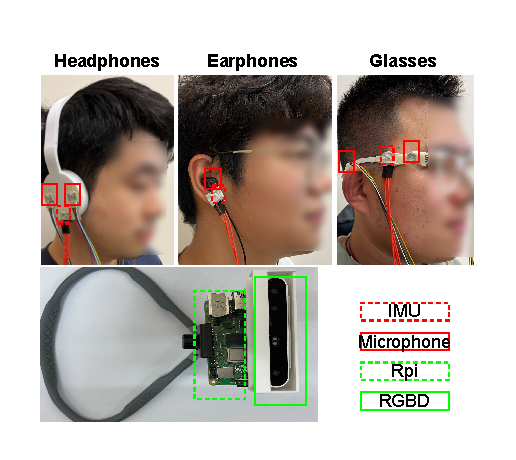
\includegraphics[width=1\linewidth]{chapters/egolog/figs/device.pdf}
    \vspace{-2em}
    \caption{Devices used in our data collection.}
    \vspace{-1em}
    \label{fig:egolog_device}
\end{figure}

\subsubsection{Public dataset}
To comprehensively evaluate EgoLog performance, we construct our dataset with the blow public datasets:

\paragraph{Ego4D:}
Ego4D \citep{grauman2022ego4d} is a large-scale dataset collected by various brands of head-mounted cameras (e.g., GoPro), offering synchronized multi-modal data (i.e., video, audio, and IMU signal). We consider the moment subset of the dataset, which consists of 158 classes. We can perform k-means clustering on the text embeddings to adapt to different levels of granularity. For the scenario annotation, we use the scenario annotation \citep{grauman2022ego4d} for each video since they have a similar definition. In total, there are 91 scenarios in the dataset. 
Considering Ego4D is the most diverse and large-scale dataset, we set it as the default dataset.

\paragraph{EgoADL:}
EgoADL \citep{sun2024multimodal} is also a large-scale dataset collected in the real world with Android smartphones, including Wi-Fi, audio, and IMU data. In this paper, we exclude Wi-Fi data for fair comparison. We perform a similar clustering for the 221 classes of actions in the dataset.

\paragraph{SAMOSA:}
SAMOSA \citep{mollyn2022samosa} is a relatively small-scale dataset collected by an Android smartwatch (i.e., Fossil Gen 5), including audio and IMU. There are 26 activities in total.

\subsubsection{Self-collected dataset}
The existing public datasets already include data from various devices—such as smart glasses, smartphones, and smartwatches—offering considerable duration and diversity. The purpose of our self-collected dataset is not to surpass these strengths but to address their limitations. Specifically, the spatial understanding discussed in Section \ref{sec:egolog_localization} relies on spatial audio, which is absent from the aforementioned datasets but is accessible using commercial devices. To compensate for this gap, we collected a new dataset featuring spatial audio recordings from different form factors: glasses, headphones, and earphones.

We constructed a dataset in which a volunteer acted as the user and a loudspeaker served as an audio interference source. The loudspeaker played audio samples from the NIGENS dataset \citep{trowitzsch2019nigens}, which contains 14 types of common sound events. The user, in contrast, performed the following 12 activities: standing up, sitting down, clapping, walking, talking, drinking, typing on a keyboard, eating, watching TV, washing hands, cleaning a room, and writing.
During data collection, the loudspeaker's position remained fixed. To simplify the experiment, the user's location was controlled for most activities (excluding walking), allowing us to manually record the relative position between the user and the loudspeaker. However, as users were not required to remain perfectly still, their precise position was not controlled with high accuracy. To ensure the dataset's validity, users were instructed to limit their positional variance to within the spatial resolution of our classification model. In essence, while the user's location was dynamic, the annotation was treated as static from the perspective of the classification task.
For the walking activity, where the relative position changes continuously, we used an RGB-D camera to perform Simultaneous Localization and Mapping (SLAM) to estimate the user's trajectory. This estimation was based on the assumption that the user started from a fixed, known position in the room (the location of the loudspeaker is also fixed and known).


\subsubsection{Baselines}
We adopt the following evaluation metrics in this paper. For the multi-label classification (i.e., scenario and spatial), we use the multi-label F1-Score: $2*TP/(2*TP+FP+FN)$. For the single-label classification (i.e., activity), we use the accuracy as the metric.

To evaluate our approach, EgoLog, we have selected different baselines for activity recognition and scenario recognition, respectively. Specifically, we consider SAMoSA \citep{mollyn2022samosa} and Imagebind \citep{girdhar2023imagebind} as our baselines for activity recognition, which are conventional supervised multi-modal model that accepts both audio and IMU. For the scenario recognition, both of the above baselines with larger data duration are considered. To ensure a fair comparison, all of them are fine-tuned with the same data.

\subsection{Activity Recognition}
\begin{figure}[h]
    \centering
    \begin{minipage}{0.48\linewidth}
        \centering
      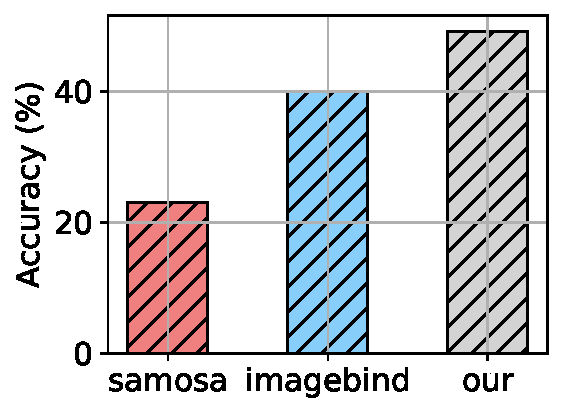
\includegraphics[width=1\linewidth]{chapters/egolog/eval/activity_ego4d.pdf}
          \vspace{-0.5em}
      \caption{Activity recognition on Ego4D.}
        \label{fig:egolog_activity_ego4d}
    \end{minipage}
    \hfill
    \begin{minipage}{0.48\linewidth}
        \centering
    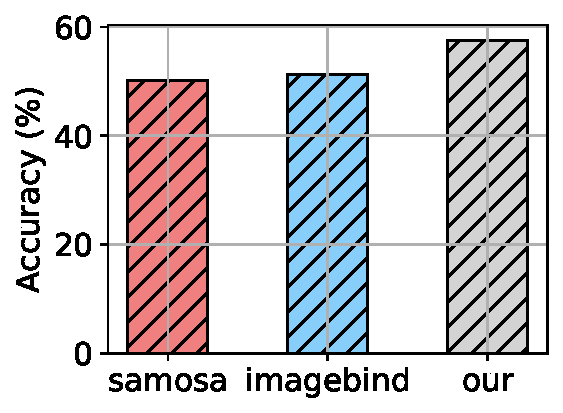
\includegraphics[width=1\linewidth]{chapters/egolog/eval/activity_egoadl.pdf}
        \vspace{-0.5em}
      \caption{Activity recognition on EgoADL.}
        \label{fig:egolog_activity_egoadl}
    \end{minipage}
    \vspace{-0.5em}
\end{figure}

\begin{figure}[h]
    \centering
    \begin{minipage}{0.48\linewidth}
        \centering
       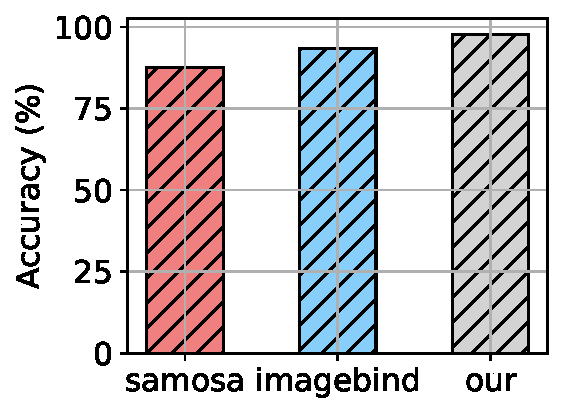
\includegraphics[width=1\linewidth]{chapters/egolog/eval/activity_samosa.pdf}
           \vspace{-0.5em}
      \caption{Activity recognition on SAMOSA.}
        \label{fig:egolog_activity_samosa}
    \end{minipage}
    \hfill
    \begin{minipage}{0.48\linewidth}
        \centering
    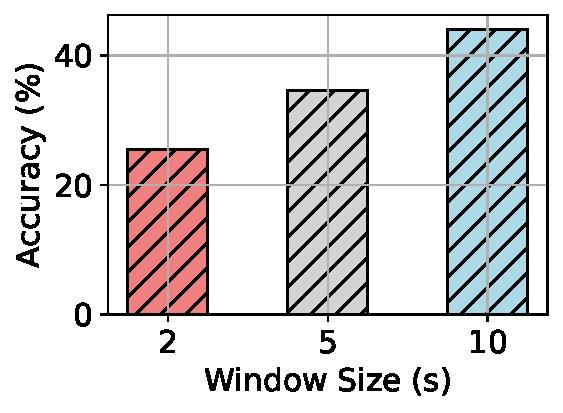
\includegraphics[width=1\linewidth]{chapters/egolog/eval/activity_window_size.pdf}
        \vspace{-0.5em}
      \caption{Activity recognition vs. data length.}
        \label{fig:egolog_activity_length}
    \end{minipage}
\vspace{-0.5em}
\end{figure}

We present the performance of our method for human activity recognition on the Ego4D, EgoADL, and SAMOSA datasets. As shown in Fig. \ref{fig:egolog_activity_ego4d}, \ref{fig:egolog_activity_egoadl}, and \ref{fig:egolog_activity_samosa}, our approach consistently outperforms the baselines, with the most notable improvement on the SAMOSA dataset.

The performance gap is most significant on the Ego4D dataset (23\% vs. 52\%), which is the most challenging. Compared to ImageBind, EgoLog achieves superior performance (52\% vs. 40\%) with significantly lower computational cost.

On the other two, less diverse datasets, the advantages of EgoLog are slightly reduced. We attribute this primarily to a lack of contextual information; Ego4D data was collected "in the wild," while the others were gathered in moderately controlled experimental settings. Despite this, our approach still outperforms the best baseline by 6\%on EgoADL and 4\%on SAMOSA, demonstrating its robustness. Note that the absolute accuracy for SAMOSA is the highest, which is expected as it has the smallest number of classes, making it the least challenging dataset.


\paragraph{Data length.}
Since the length of the data significantly influences both audio and IMU data, we first establish the hyperparameters before evaluating the system.
We present the performance of human activity recognition along with various data lengths, in Fig. \ref{fig:egolog_activity_length}. We observe that the HAR performance stays stable when the data length is larger than five seconds, while significantly dropping when the data length is one second. As a result, we keep the data length of HAR to five seconds. 

\begin{figure}[h]
    \centering
    \begin{minipage}{0.48\linewidth}
        \centering
       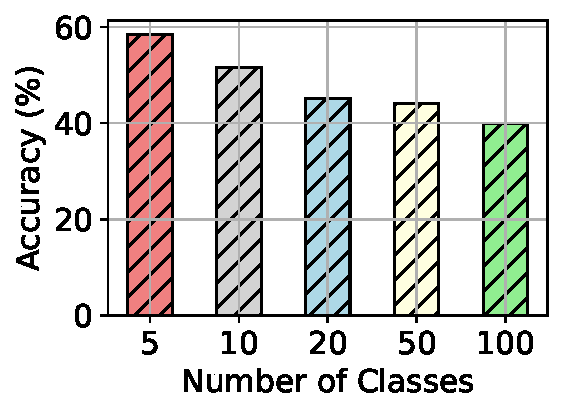
\includegraphics[width=1\linewidth]{chapters/egolog/eval/activity_num_classes.pdf}
           \vspace{-0.5em}
      \caption{Human activities recognition performance vs. number of classes.}
        \label{fig:egolog_activity_num_classes}
    \end{minipage}
    \hfill
    \begin{minipage}{0.48\linewidth}
        \centering
    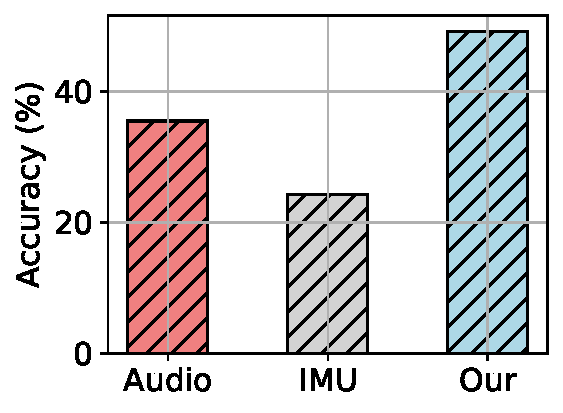
\includegraphics[width=1\linewidth]{chapters/egolog/eval/activity_modality.pdf}
        \vspace{-0.5em}
      \caption{Human activities recognition performance vs. modality.}
        \label{fig:egolog_activity_modality}
    \end{minipage}
\vspace{-0.5em}
\end{figure}

\paragraph{Number of classes.}
We split the sampled Ego4D dataset into activities and evaluated their performance in Fig. \ref{fig:egolog_activity_num_classes}. We observe that there are performance gaps between activities, indicating that the complexity of each of them is different. Specifically, we inspect the top three worst activities, which are putting something in a container or on a surface, cutting with scissors, and sleeping. We observe that they are both quiet, and the motion is weakly related to the head, so it is natural to have lower performance.

\paragraph{Modalities fusion.}
As shown in Figure \ref{fig:egolog_activity_modality}, our multi-modal fusion approach (audio+IMU) surpasses the audio-only and IMU-only baselines, improving activity recognition performance by more than 10\%.


\begin{table}[h]
\centering
\caption{Ablation study on activity recognition for different datasets, the metric is accuracy.}
\label{tab:ab_activity}
\begin{tabular}{ccccc}
\toprule
\textbf{Model}  & \textbf{Ego4D$\uparrow$} & \textbf{EgoADL$\uparrow$} & \textbf{SAMOSA$\uparrow$} \\
\midrule
Random  & 0.02 & 0.02 & 0.04 \\
\midrule
ImageBind-FT  & 0.40 & 0.51 & 0.93 \\
\midrule
Multi-modal & 0.401 & 0.49 & 0.90\\
+ Scenario & \textbf{0.467} & \textbf{0.58} & \textbf{0.97} \\
\bottomrule
\end{tabular}
\end{table}

\paragraph{Ablation study.}
We conduct an ablation study on different components of our system, including each modality (audio and IMU), multi-modal fusion, scenario as condition, and scenario as condition via Imagebind-embedding, as shown in Tab. \ref{tab:ab_activity}. For reference, we also list the performance of a random guess (indicating the number of classes) and baseline ImageBind-FT.
We observe that


\subsection{Scenario Recognition}
\begin{figure}[h]
    \centering
    \begin{minipage}{0.48\linewidth}
        \centering
    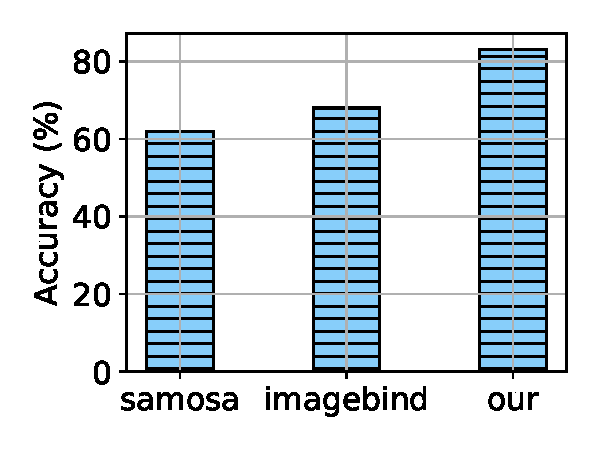
\includegraphics[width=1\linewidth]{chapters/egolog/eval/scenario_cls.pdf}
           \vspace{-0.5em}
      \caption{Scenario recognition accuracy on Ego4D.}
        \label{fig:egolog_scenario}
    \end{minipage}
    \hfill
    \begin{minipage}{0.48\linewidth}
        \centering
    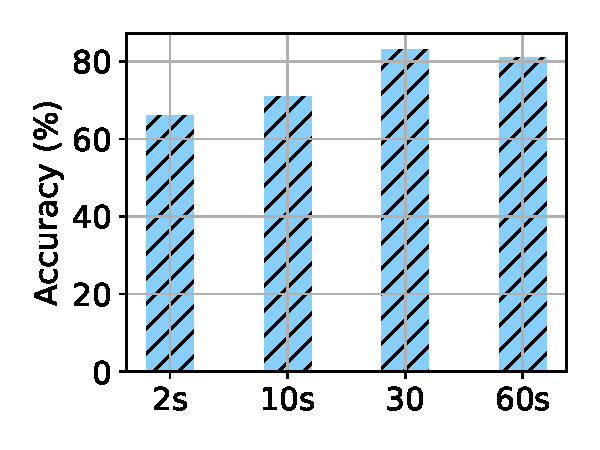
\includegraphics[width=1\linewidth]{chapters/egolog/eval/scenario_length.pdf}
        \vspace{-0.5em}
      \caption{Scenario recognition accuracy vs. data length.}
        \label{fig:egolog_scenario_length}
    \end{minipage}
    \vspace{-0.5em}
\end{figure}



\begin{figure}[h]
    \centering
    \begin{minipage}{0.48\linewidth}
        \centering
      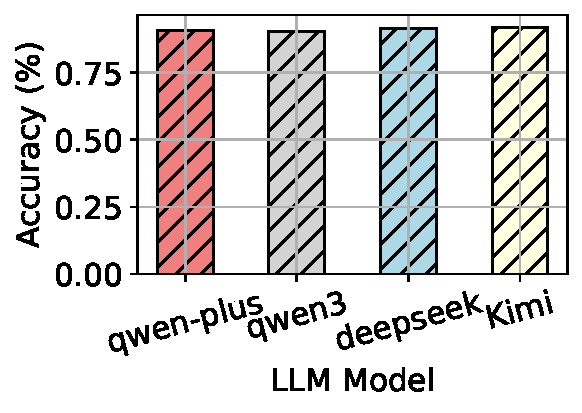
\includegraphics[width=\linewidth]{chapters/egolog/eval/scenario_llm_model.pdf}
          \vspace{-0.5em}
     \caption{Selection of LLM.}
    \label{fig:egolog_selection_llm}
    \end{minipage}
    \hfill
    \begin{minipage}{0.48\linewidth}
     \begin{tabular}{cc}
        \toprule
        \textbf{Model} & \textbf{Ego4D$\uparrow$} \\
        \midrule
        Random & 0.01\\
        \midrule
        Multi-modal & 0.70 \\
        + Contrastive & 0.83\\
        + Transformer  & 0.85 \\
        + LLM feedback  & 0.90\\
        \bottomrule
        \end{tabular}
        \vspace{1em}
        \captionof{table}{Ablation study on scenario recognition.}
        \label{tab:ab_scenario}
    \end{minipage}
    \vspace{-0.5em}
\end{figure}


Recalled in Sec. \ref{sec:egolog_scenario}, we employ a two-stage model to recognize the scenario by extracting the key-frame. In comparison, we consider audio scene recognition and ImageBind-IMU, which are audio-only and IMU-only methods
as the two baselines shown in Fig. \ref{fig:egolog_scenario}. We observe that our method outperforms the two baselines by 15\%, indicating that our long-time multi-modal fusion works well for scenario recognition. 

\paragraph{Data length.}
Based on our earlier definitions, scenarios that require capturing long-term information should use longer data lengths. We present the performance of scenario recognition along with various data lengths in Fig. \ref{fig:egolog_scenario_length}. We observe that the ideal data length is set to 30 seconds since the larger input data can reduce the performance.

\paragraph{Selection of LLM.}
Since our design is compatible with any LLM, we evaluated the performance using different LLMs from various sources. As shown in Fig. \ref{fig:egolog_selection_llm}, we observe that the performance is similar across them, indicating that common LLMs are sufficient for our design. For better deployment, we plan to explore the use of smaller LLMs in the future to reduce costs.

\paragraph{Ablation study.}
We conducted an ablation study to evaluate the contribution of different components in our system, including contrastive learning, the transformer module, and the addition of LLM feedback. The results are presented in Tab. \ref{tab:ab_scenario}. For reference, we also include the performance of a random guess (based on the number of classes).

Our observations indicate that contrastive learning is the most effective component, providing the largest performance improvement (13\%). The LLM feedback, facilitated by edge-cloud collaboration, yields a further, albeit smaller, gain. Given that LLM feedback is less susceptible to cross-domain variations, we consider this slight improvement to be meaningful.



\subsection{Spatial Understanding for Scenario Recognition}
\begin{figure}[h]
    \centering
    \begin{minipage}{0.48\linewidth}
         \centering
    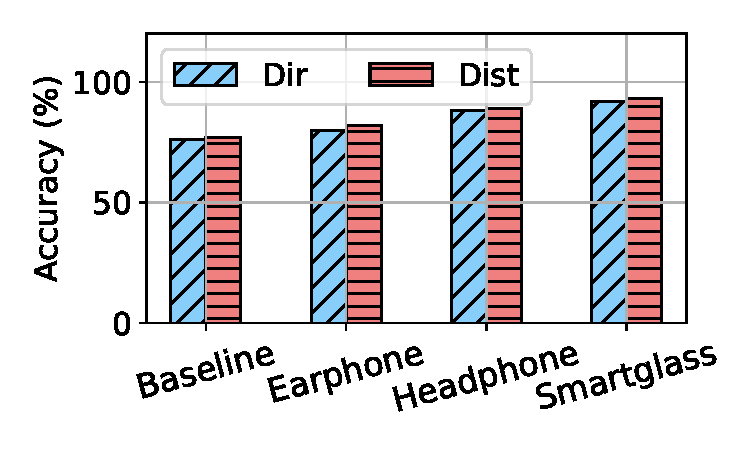
\includegraphics[width=1\linewidth]{chapters/egolog/eval/sound_localization.pdf}
            \vspace{-0.5em}
      \caption{Sound localization accuracy.}
        \label{fig:egolog_sound_localization}
    \end{minipage}
    \hfill
    \begin{minipage}{0.48\linewidth}
        \centering
    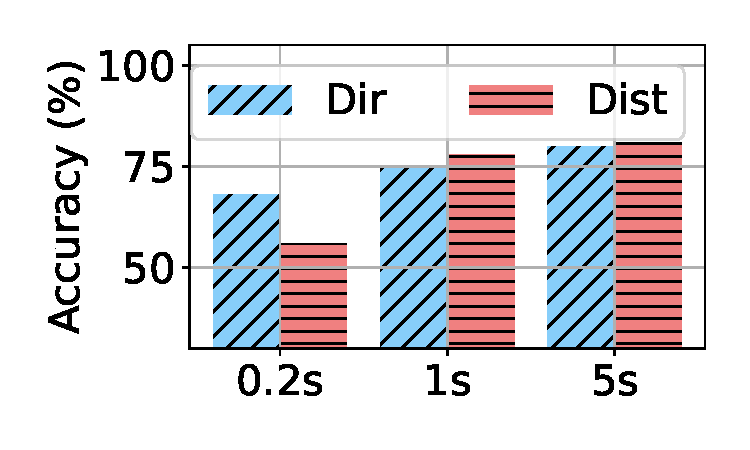
\includegraphics[width=1\linewidth]{chapters/egolog/eval/sound_localization_length.pdf}
          \vspace{-0.5em}
    \caption{Sound localization accuracy vs. data length.}
    \label{fig:egolog_sound_localization_length}
    \end{minipage}
    \vspace{-0.5em}
\end{figure}

\begin{figure}[h]
  \centering
  \begin{minipage}{0.4\linewidth}
    \centering
    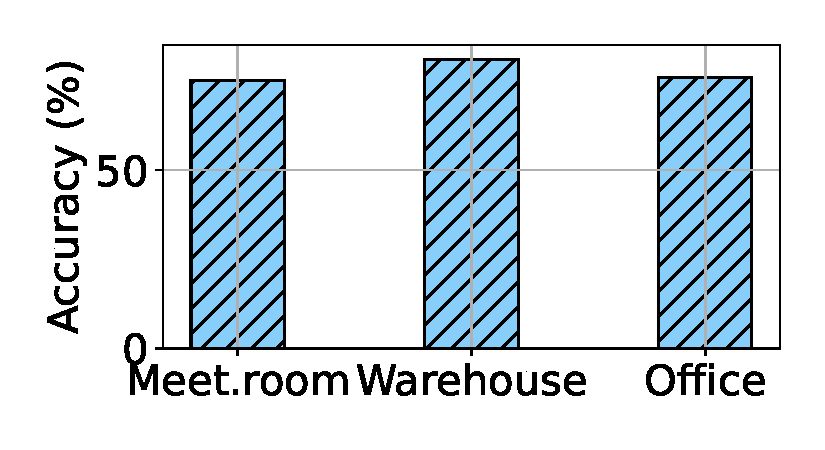
\includegraphics[width=1\linewidth]{chapters/egolog/eval/sound_localization_place.pdf}
        \vspace{-0.5em}
      \caption{Sound localization accuracy at different places.}
        \label{fig:egolog_sound_localization_place}
  \end{minipage}
  \hfill
  \begin{minipage}{0.58\linewidth}
    \centering
     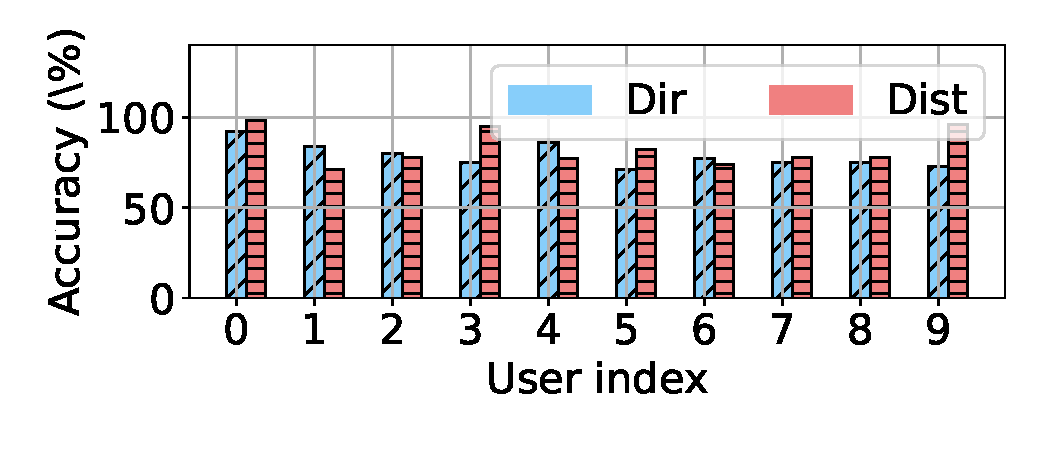
\includegraphics[width=1\linewidth]{chapters/egolog/eval/sound_localization_user.pdf}
         \vspace{-0.5em}
      \caption{Binaural sound localization accuracy for different users.}
        \label{fig:egolog_sound_localization_user}
  \end{minipage}
\vspace{-0.5em}
\end{figure}
In Fig. \ref{fig:egolog_sound_localization}, we compare the baseline (without motion compensation) with our proposed method across different devices. We report the accuracy for both direction (Dir) and distance (Dist) separately. The results show that our method improves accuracy by approximately 10\%when using IMU data for motion compensation.

Regarding performance across devices, we observe a consistent improvement from binaural earphones to 4-channel headphones and further to 4-channel smart glasses, which aligns with our expectations. In the following section, we will focus on evaluating data from earphones, which exhibit the lowest performance.

\paragraph{Data length.}
Since the length of the audio significantly influences the performance of sound localization, we test the accuracy with different length of data in Fig. \ref{fig:egolog_sound_localization_length}. According to the result, we set the data length of sound localization to one second to balance the latency and accuracy.

\paragraph{Different environments.}
We conducted further assessments of localization accuracy across various environments, such as distinct rooms. Room layout and object configurations induce varying room impulse responses, affecting recordings in conjunction with HRTFs. Our performance evaluation across different rooms is presented in Figure \ref{fig:egolog_sound_localization_place}, demonstrating that our model maintains consistent performance across diverse settings.

\paragraph{Different users.}
Binaural sound localization depends on individual-specific HRTFs, rendering neural networks calibrated for one user
ineffective for others. We assess personalized models across a group of users and present the overall accuracy in Figure 21. Despite performance variations among users, consistent accuracy (>75\%) is maintained within the group

\subsection{User Study}

% \begin{table}[h]
% \centering
% \vspace{-0.5em}
% \caption{User study.}
% \label{tab:user_study}
% \begin{tabular}{ll}
% \toprule
% \textbf{Question} & \textbf{EgoLog}\\
% \midrule
% Correctness &  \\
% Information-richness & \\
% User-friendly & \\
% \bottomrule
% \end{tabular}
% \vspace{-0.5em}
% \end{table}

To evaluate the benefits of EgoLog from a user perspective, we conducted a study where volunteers provided subjective ratings of the system's outputs. Recall that our goal is to provide users with a daily log that comprehensively summarizes and represents their activities through two complementary types of output: scenarios and activities. 
Our final solution integrates both outputs: the daily log displays two rows, with the first row showing scenario information and the second row presenting activity data. Since scenarios are recognized every 30 seconds, the output can contain errors or inconsistencies, even within the same scenario. To mitigate this, we represent each scenario using the normalized probability calculated from the most recent 10 minutes of data. 
For activities, due to the larger volume of data, we present the results using a bar chart with activity names labeled at the bottom.
Users were asked to rate the outputs based on three criteria: Correctness, Information-richness, and User-friendliness. To assess correctness, they were provided with ground-truth data in the same format. The average ratings (on a scale of 1-min to 5-max) for the three dimensions were 4.5, 4.0, and 4.5, respectively.


\subsection{Overhead}
While our system is not specifically designed for real-time responses, it is crucial to maintain low resource consumption.

\begin{table}[h]
\centering
\vspace{-0.5em}
\caption{Model runtime latency.}
\vspace{-0.5em}
\label{tab:latency}
\begin{tabular}{llcc}
\toprule
\textbf{Section} & \textbf{Interval} & \textbf{CPU} & \textbf{GPU} \\
\midrule
Scenario & 30 seconds & 0.55s & 9ms \\
Spatial & 2 seconds & 2.5ms & 2.1ms \\
HAR  & 10 seconds & 34ms & 2.7ms \\
\bottomrule
\end{tabular}
\vspace{-0.5em}
\end{table}

\paragraph{Latency.}
EgoLog comprises three core components: (1) scenario recognition (Sec. \ref{sec:egolog_scenario}), (2) sound localization (Sec. \ref{sec:egolog_localization}), and (3) HAR (Sec. \ref{sec:egolog_har}). As shown in Tab. \ref{tab:latency}, most components are lightweight, enabling real-time performance on both CPU and GPU platforms. Notably, scenario recognition on CPU requires 0.55 seconds but is executed once every 30 seconds, rendering its latency negligible. While EgoLog does not mandate real-time user feedback, lower latency enhances user experience by minimizing wait times.


\paragraph{Power consumption.}
To evaluate our power consumption, we locked the screen while continuously recording both audio and IMU data. We then checked the battery level before and after one hour of recording. Using the Pixel 7 as a reference, we observed approximately a 5\% drop in power after one hour of recording. Given that there is potential for further optimization, EgoLog shows promise for effective long-term operation.

\paragraph{Data storage.}
We record audio at a sample rate of 48 kHz, with a 16-bit depth and 2 channels, resulting in a compressed file size of about 170-210 kbps in MP3 format. This equates to around 70 MB of audio data per hour. For motion data, with an update rate set to 10 Hz, the size in CSV format is approximately 1 kB per second, leading to around 3 MB of data per hour.
As a result, we can process this data periodically, ensuring that storage requirements remain manageable and do not become overwhelming.



